\subsection{Diagrammes de classes}
Les diagrammes de classes suivants sont disponibles dans le dépôt des Livrables pour une meilleure qualité.\\


\textbf{Diagramme de classe du package racine du projet.}\\
\begin{center}
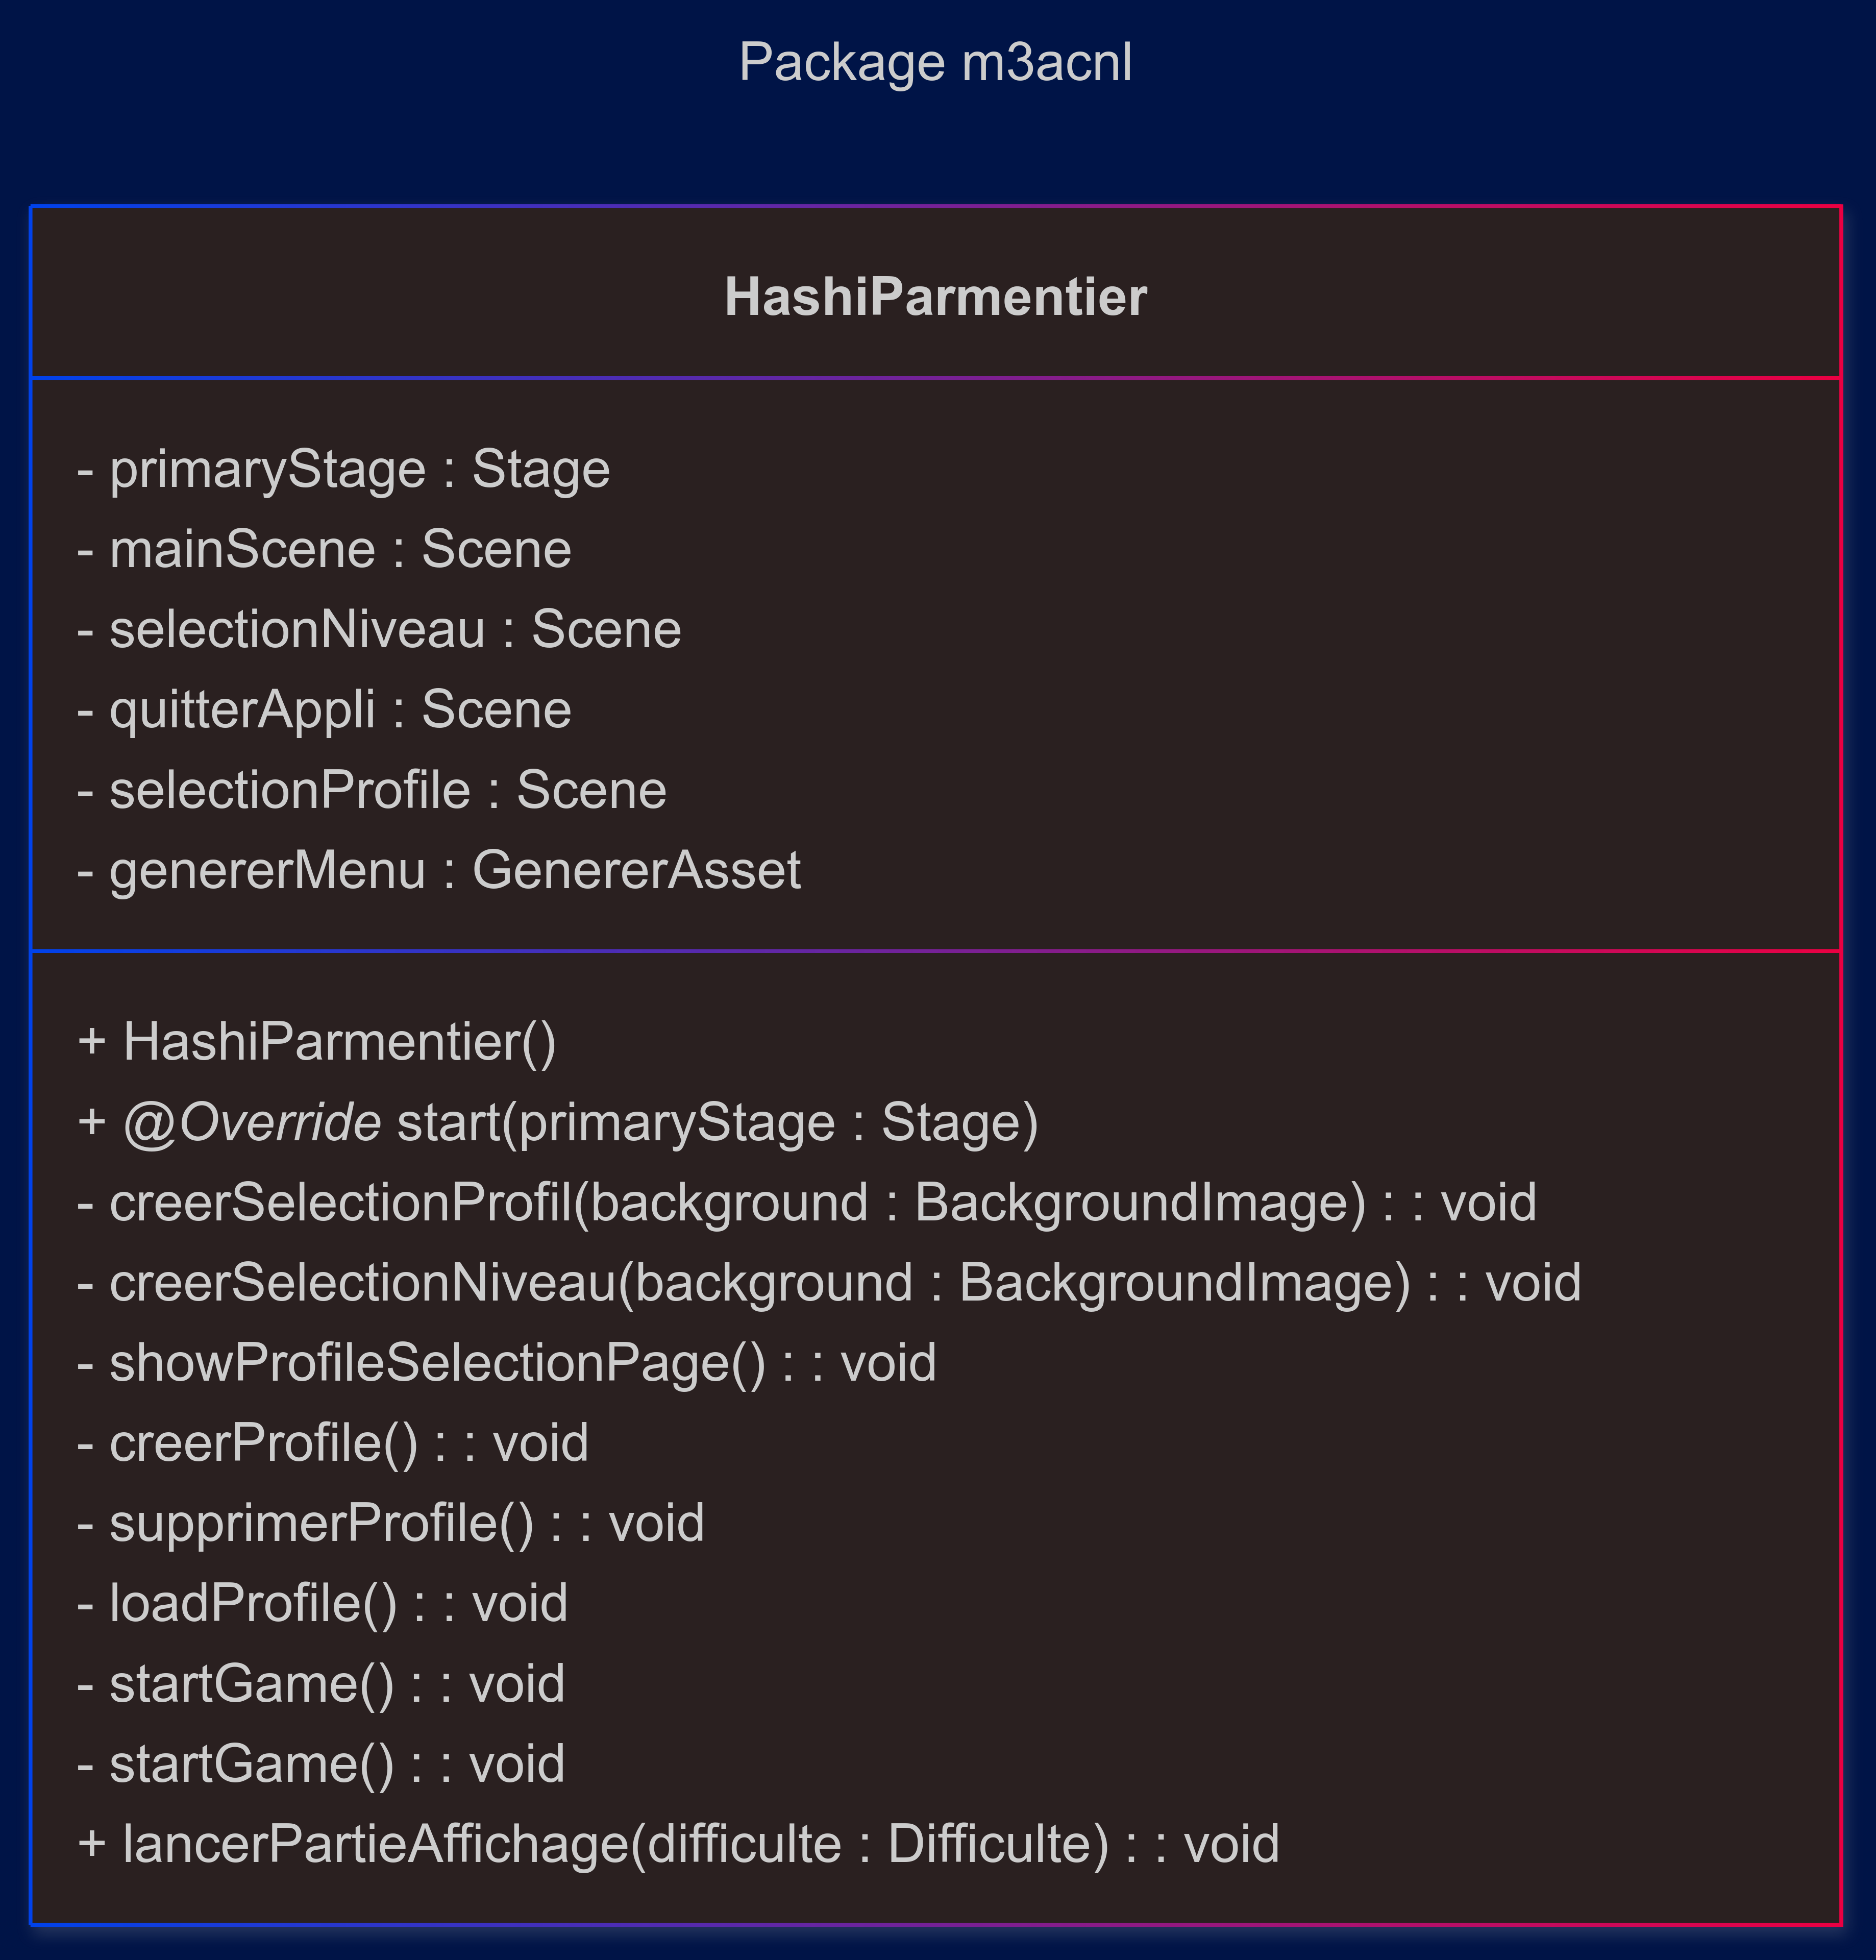
\includegraphics[width=\textwidth,height=\dimexpr\textheight-220pt\relax,keepaspectratio]{../Annexe/classes/HashiParmentier.png}
\end{center}

\pagebreak

\textbf{Diagramme de classe du package du jeu.}\\
\begin{center}
    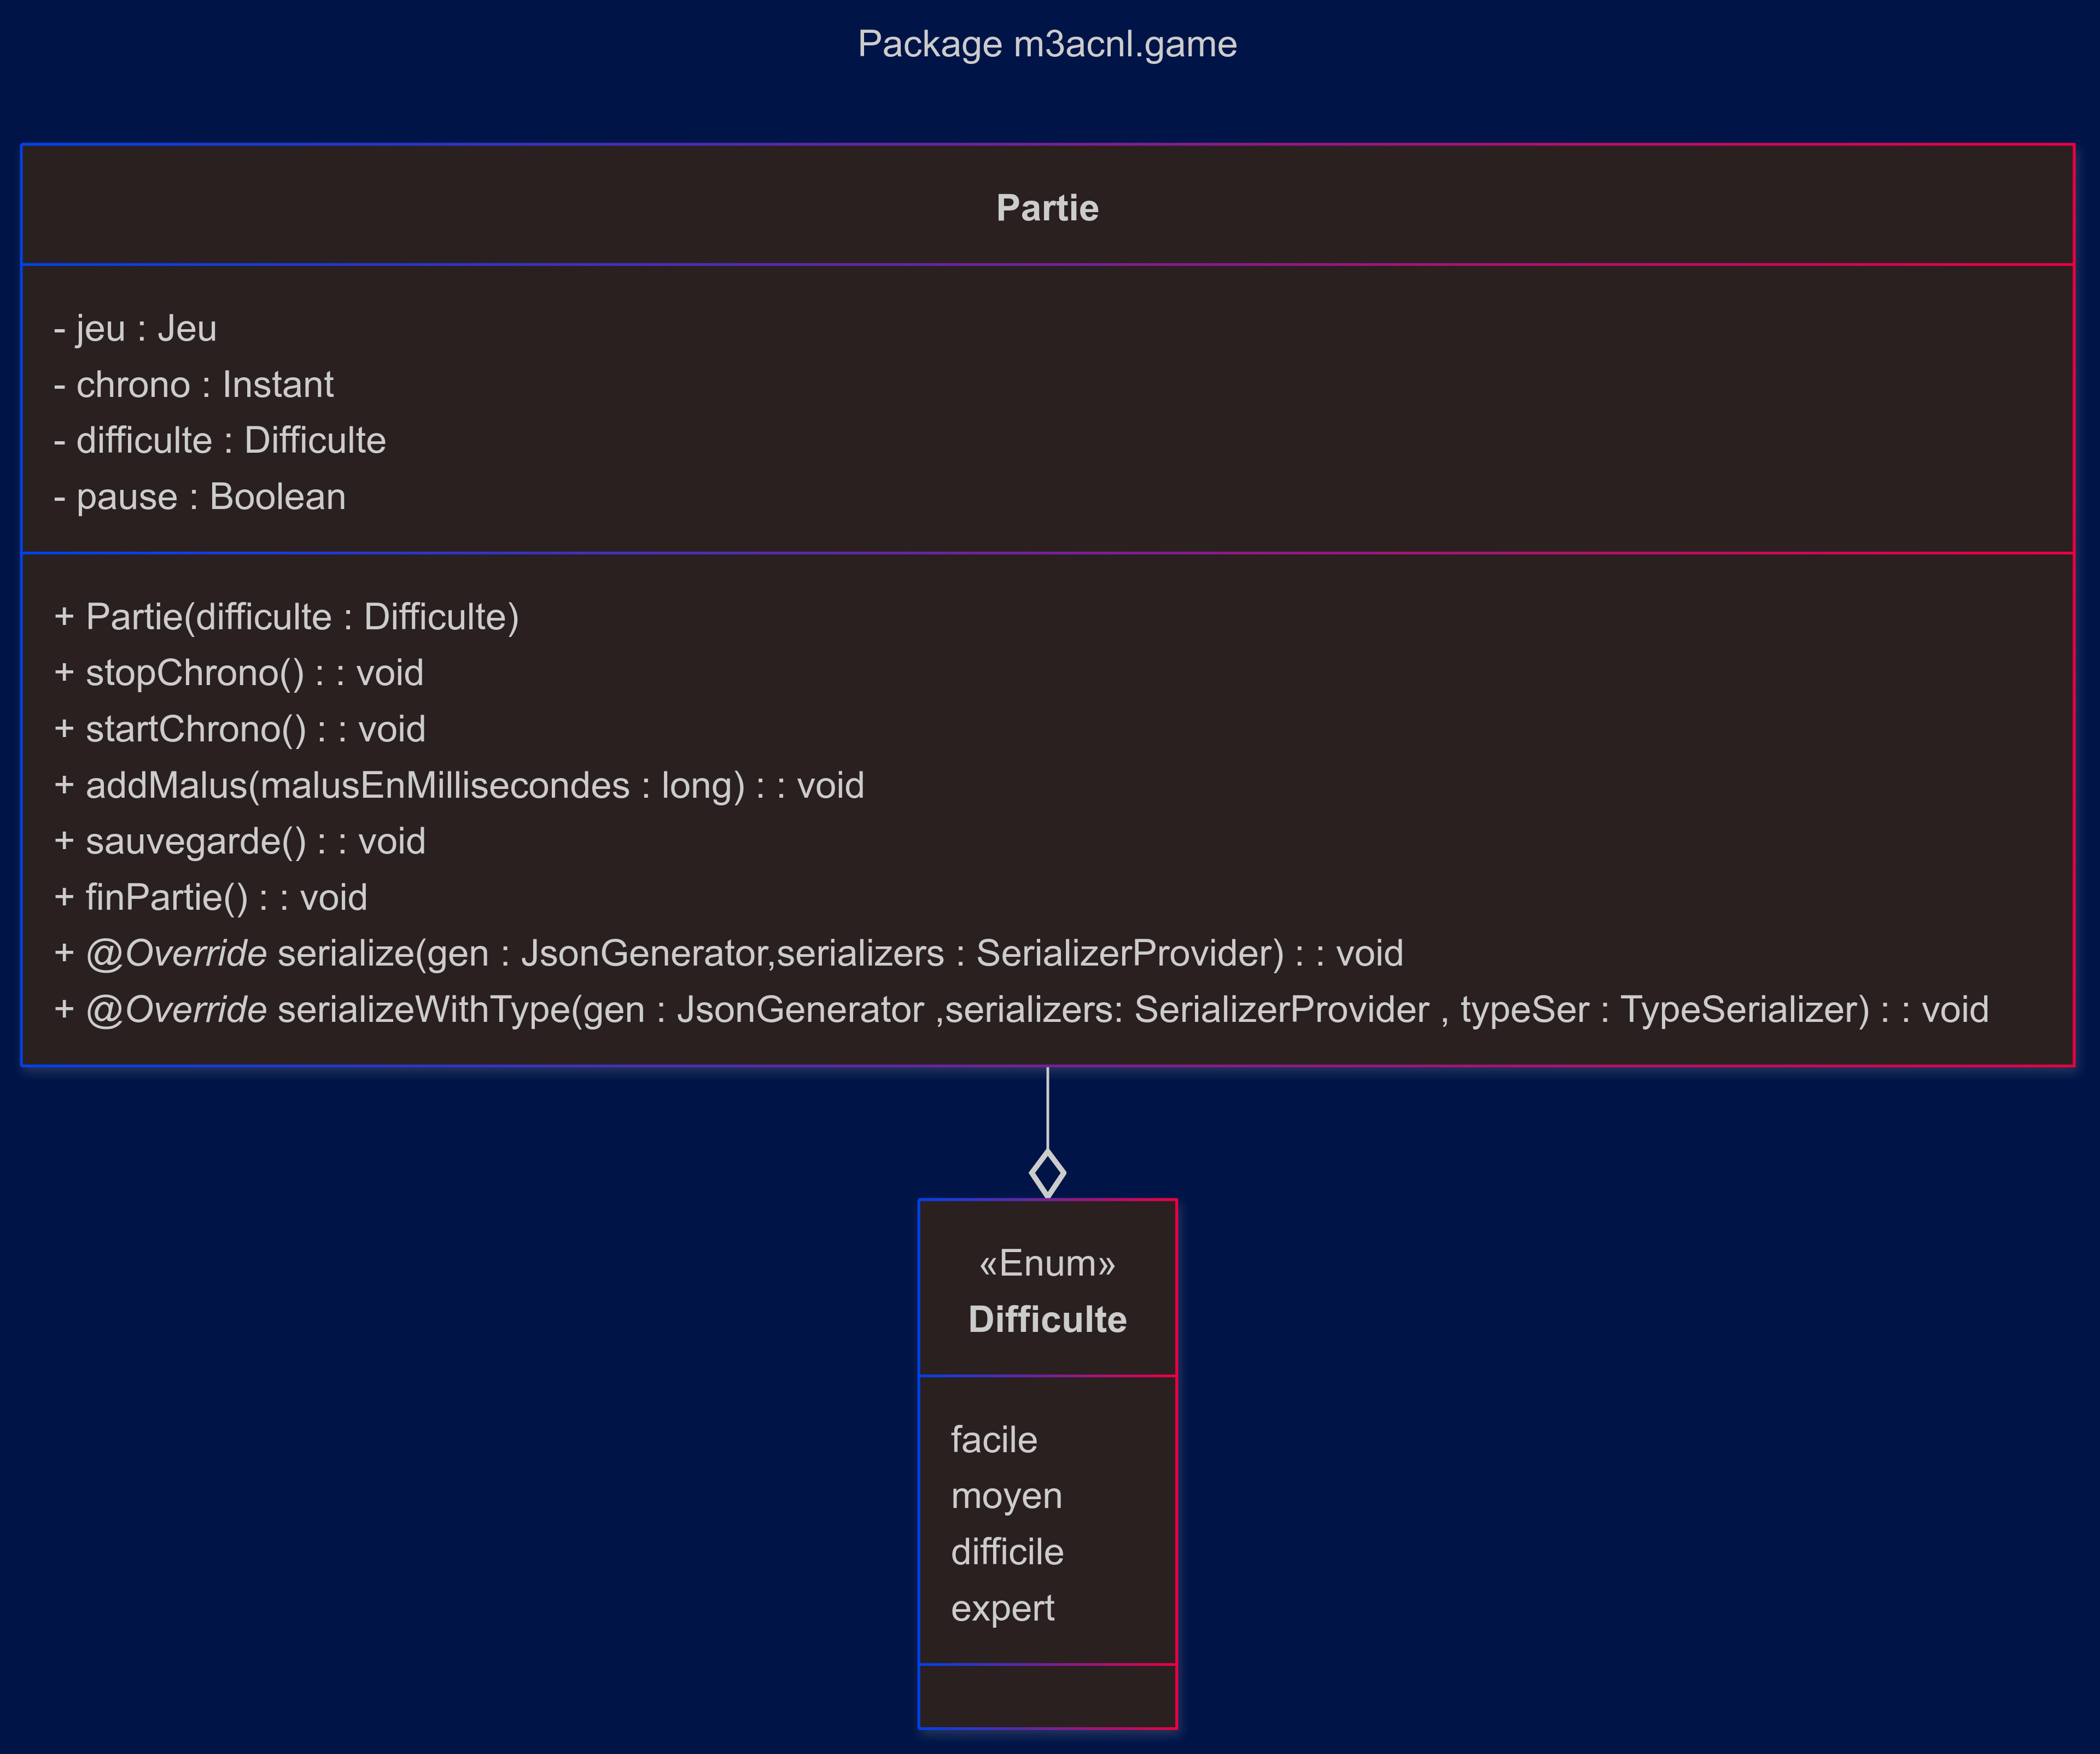
\includegraphics[width=\textwidth,height=\textheight,keepaspectratio]{../Annexe/classes/game.png}
\end{center}

\pagebreak

\textbf{Diagramme de classe de la partie graphique.}\\
\begin{center}
    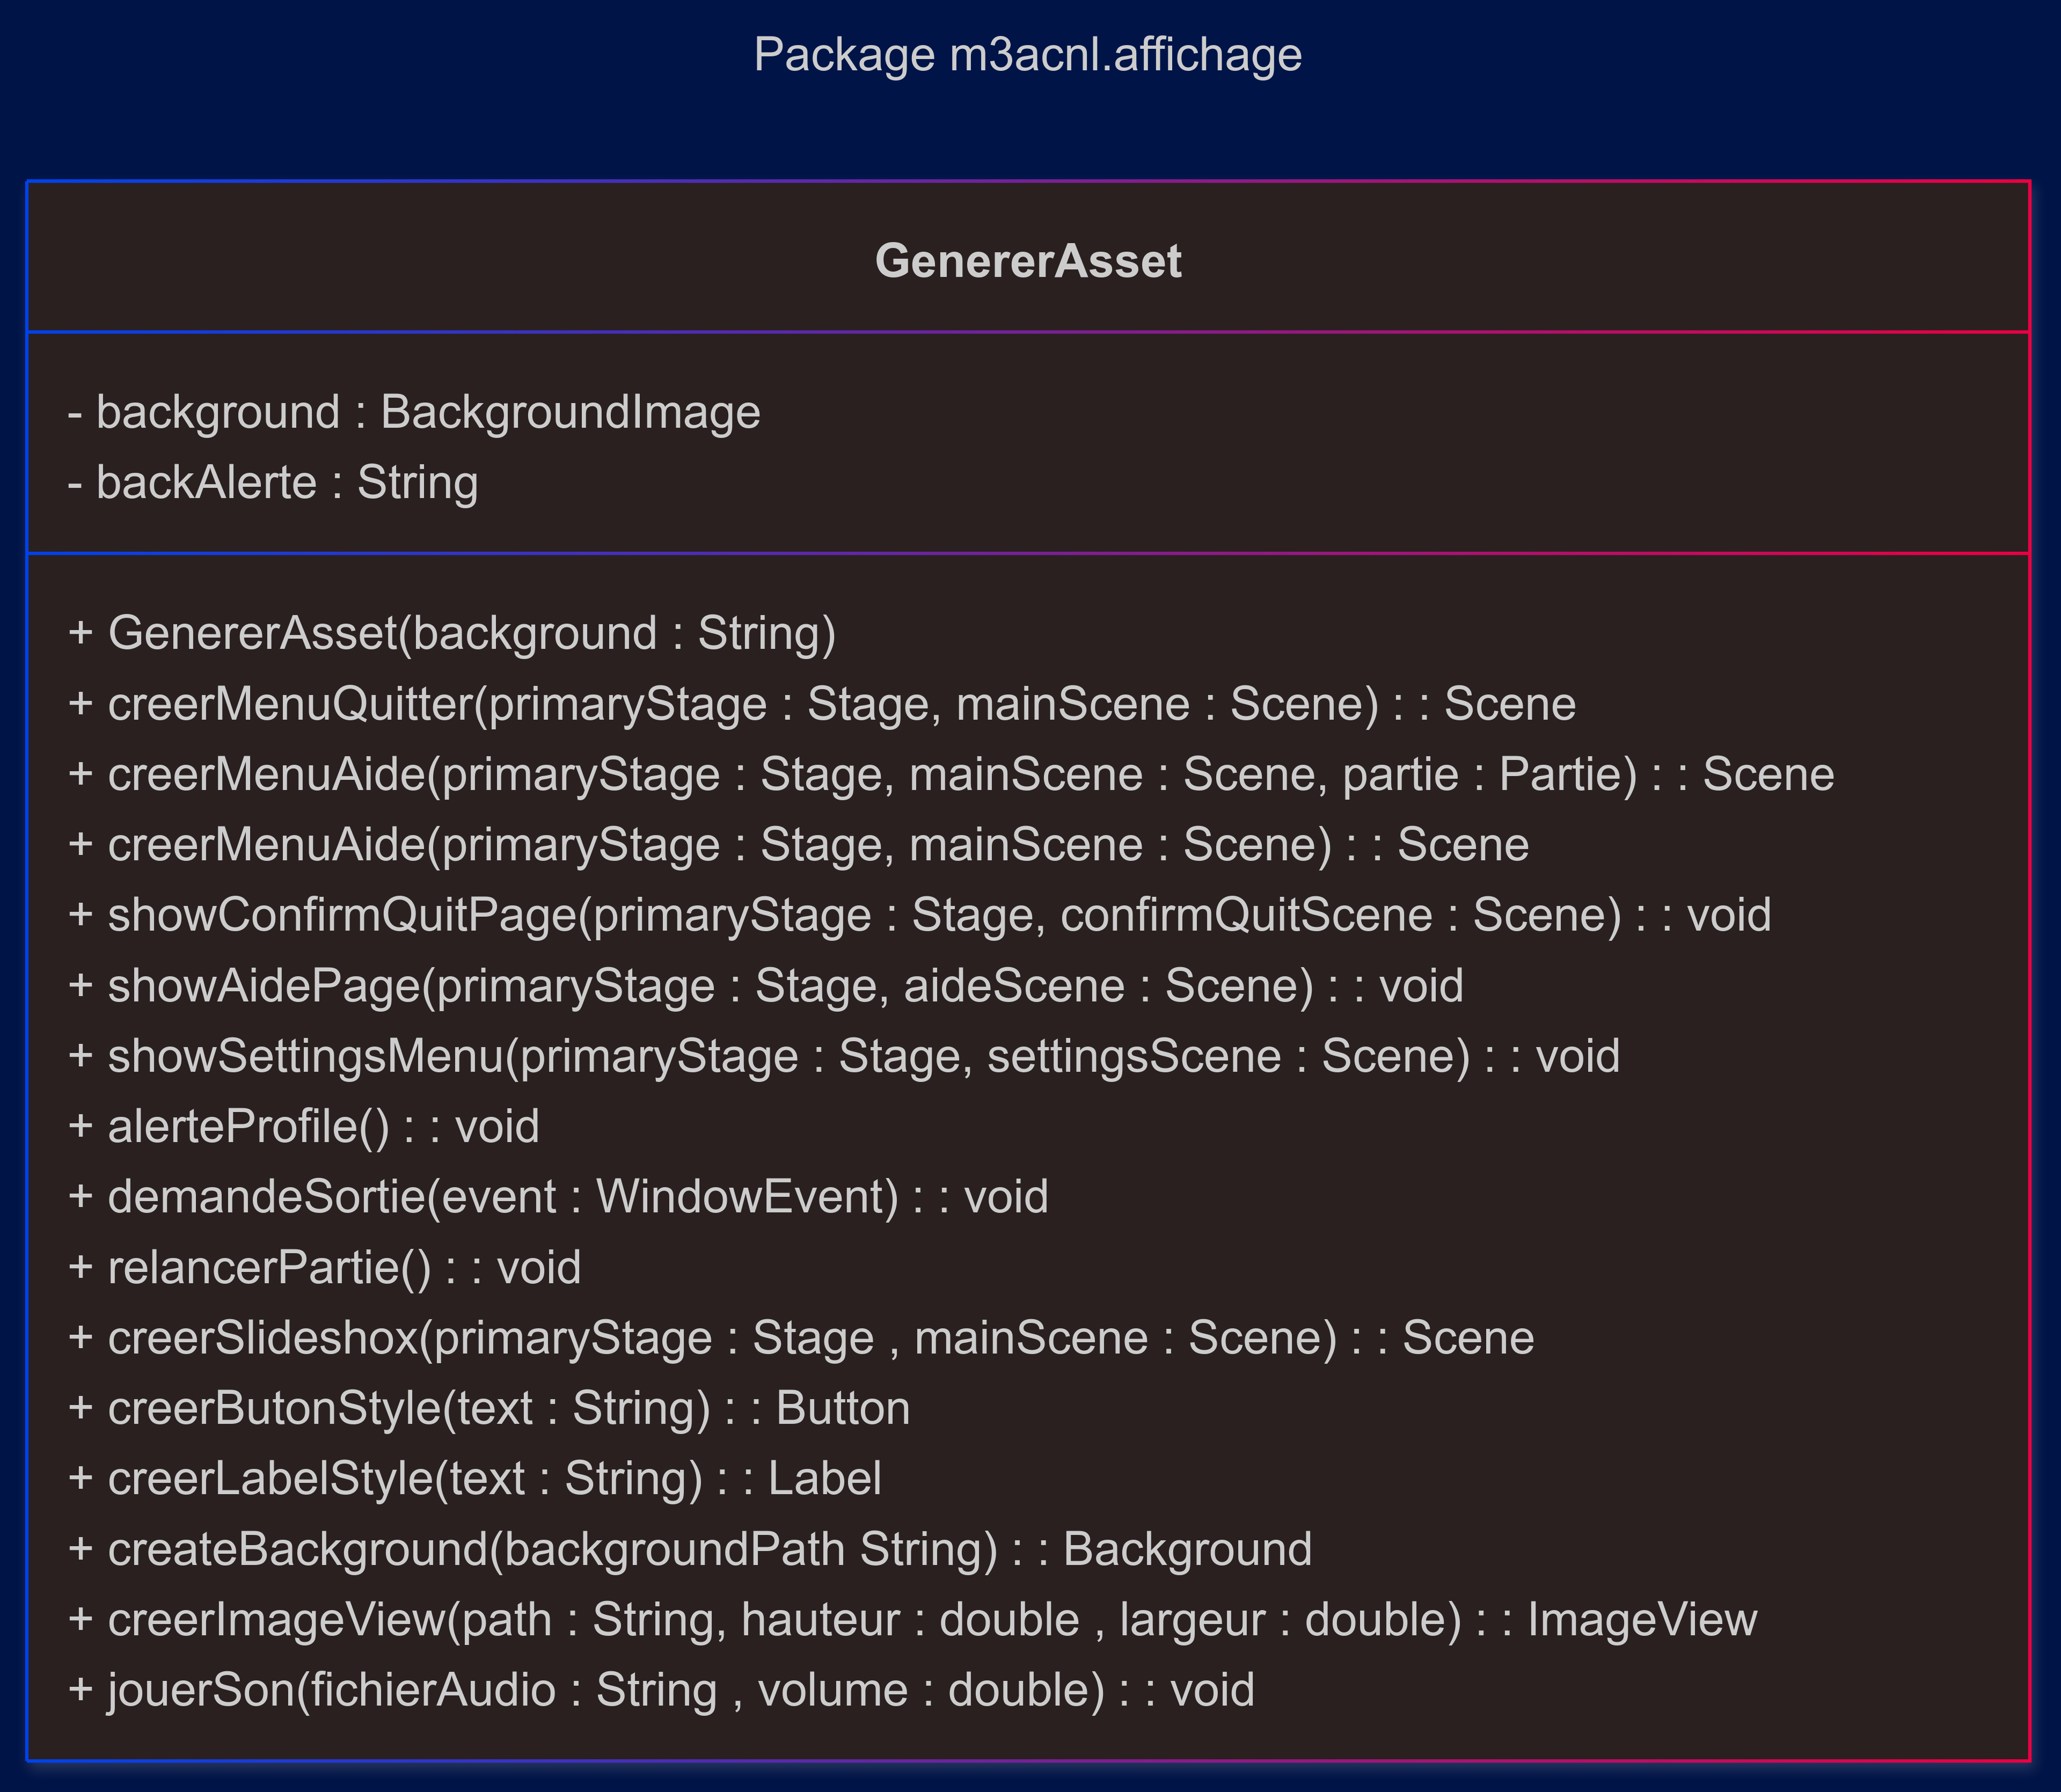
\includegraphics[width=\textwidth,height=\textheight,keepaspectratio]{../Annexe/classes/affichage.png}
\end{center}

\pagebreak

\textbf{Diagramme de classe de la partie graphique et partie logique.}\\
\begin{center}
    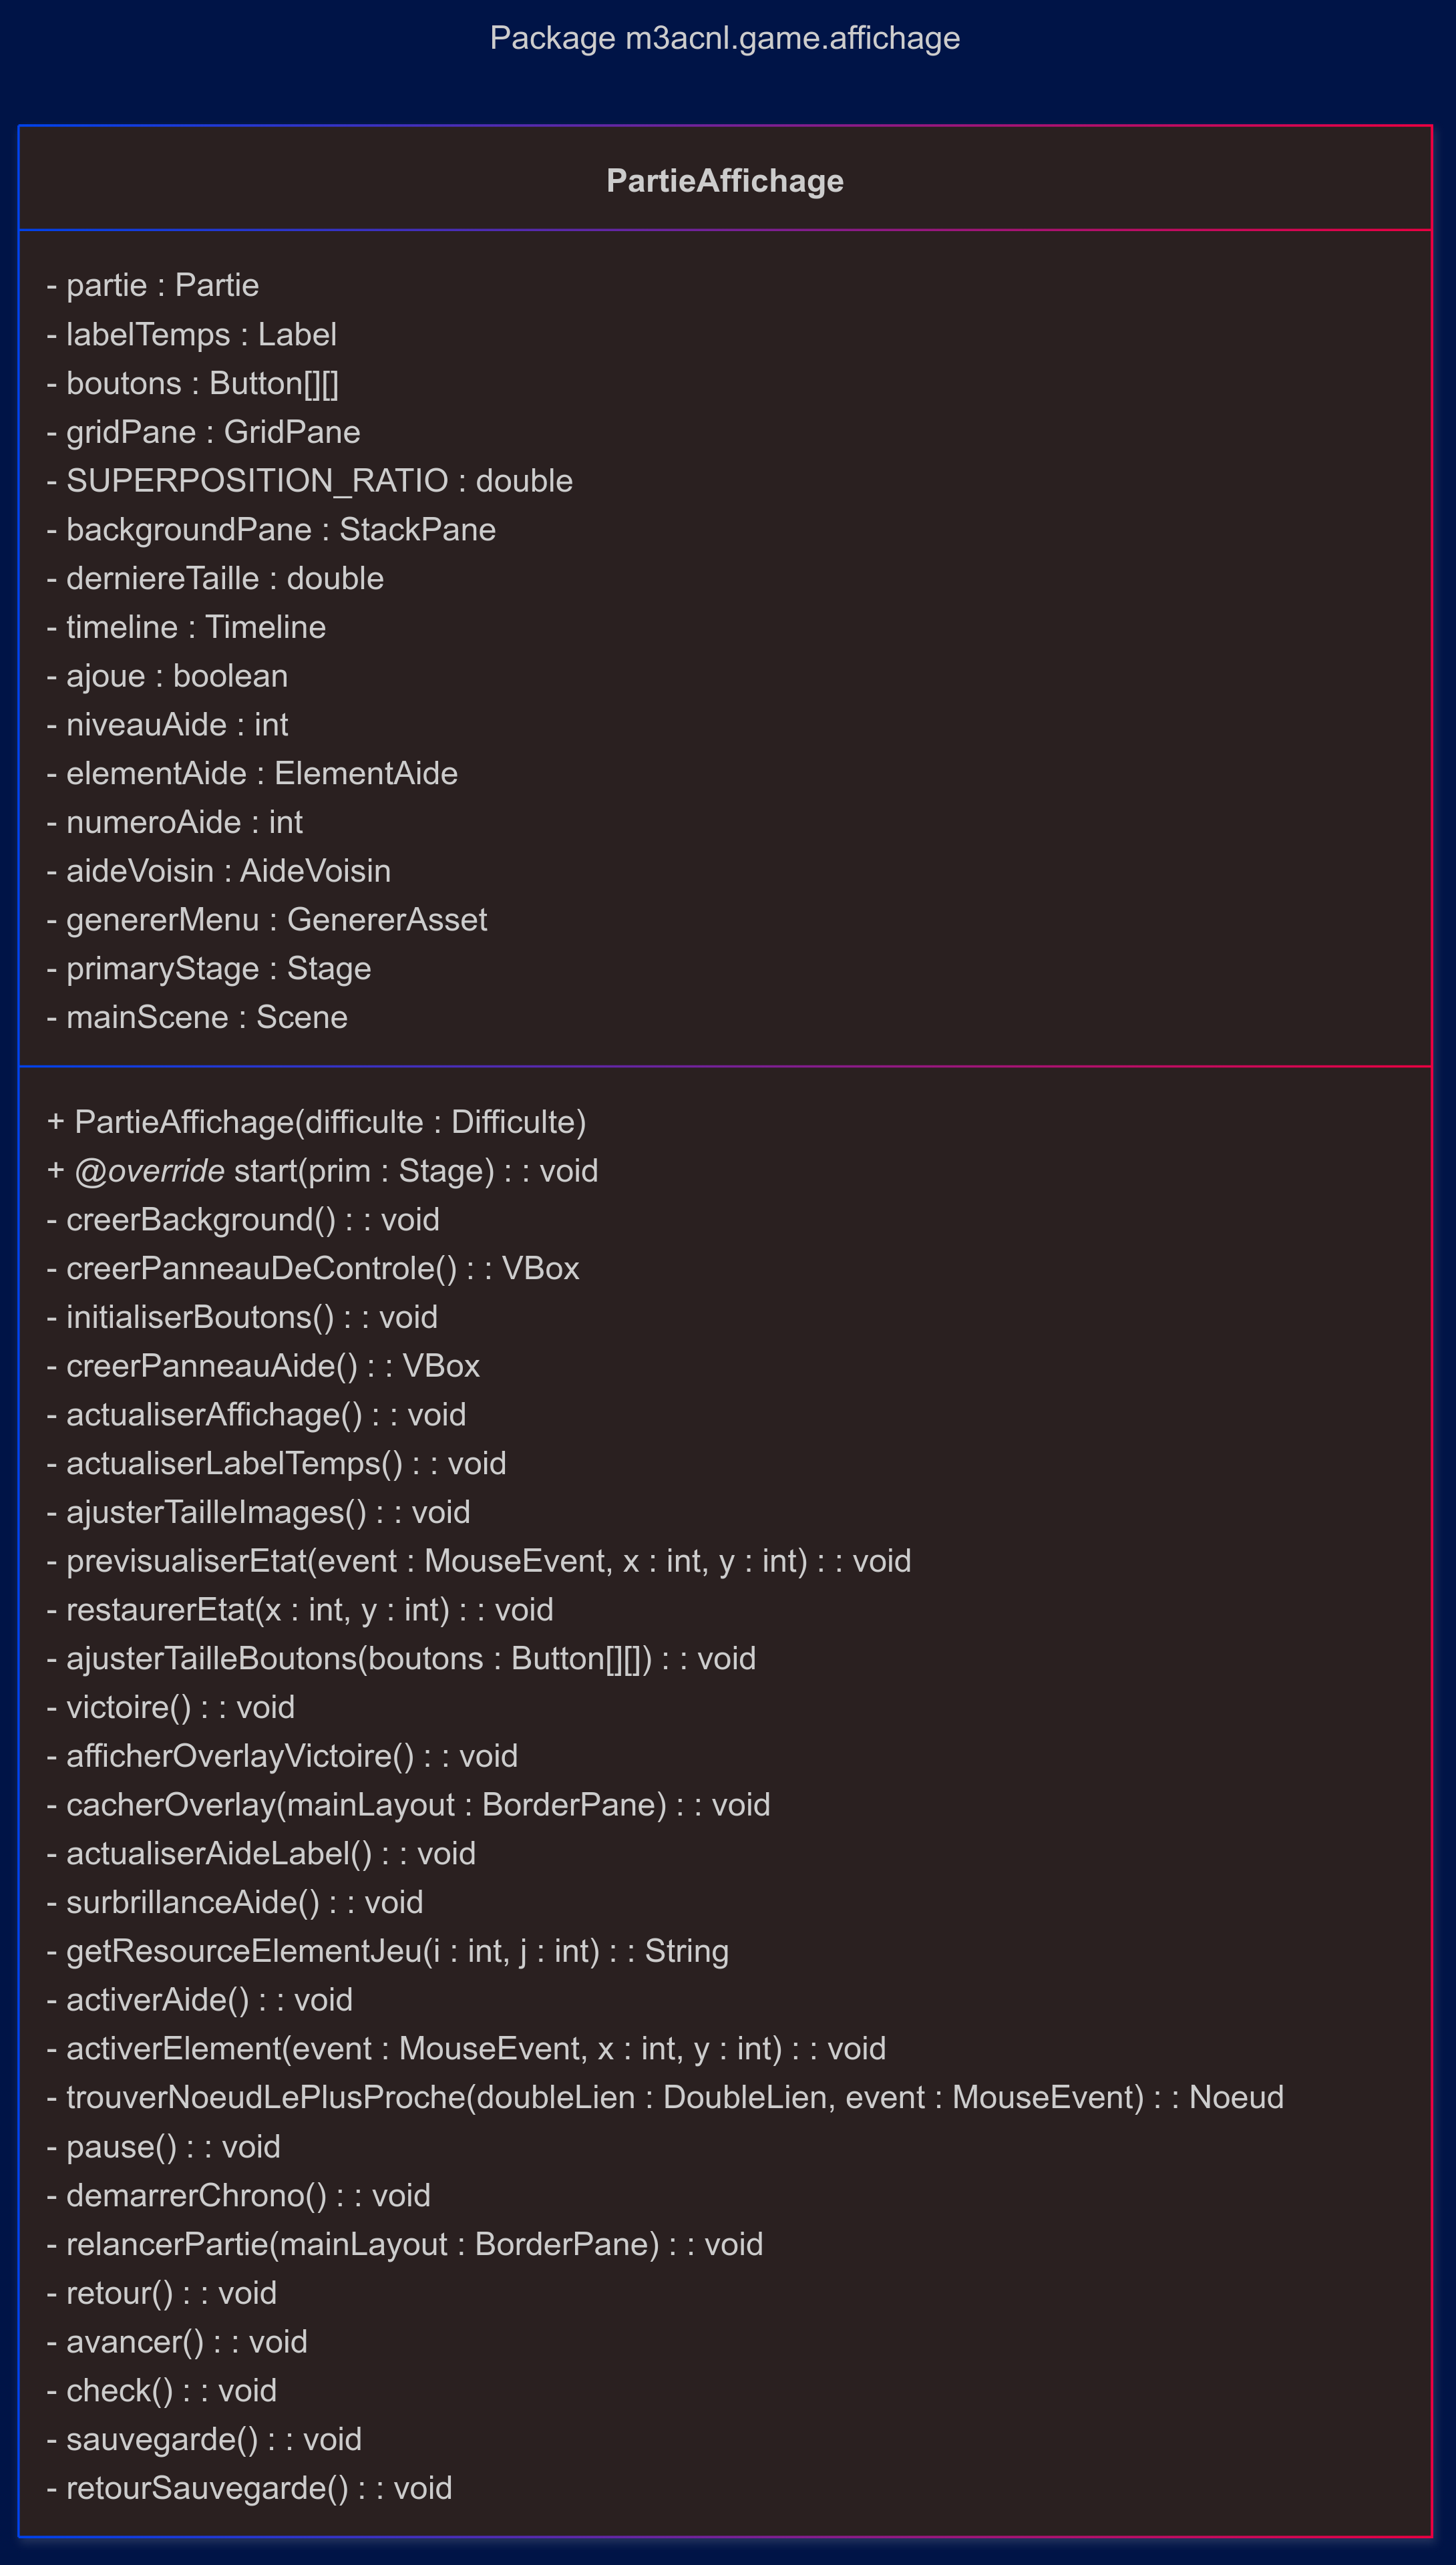
\includegraphics[width=\textwidth,height=\dimexpr\textheight-40pt\relax,keepaspectratio]{../Annexe/classes/gameAffichage.png}
\end{center}

\pagebreak

\textbf{Diagramme de classe des managers.}\\
\begin{center}
    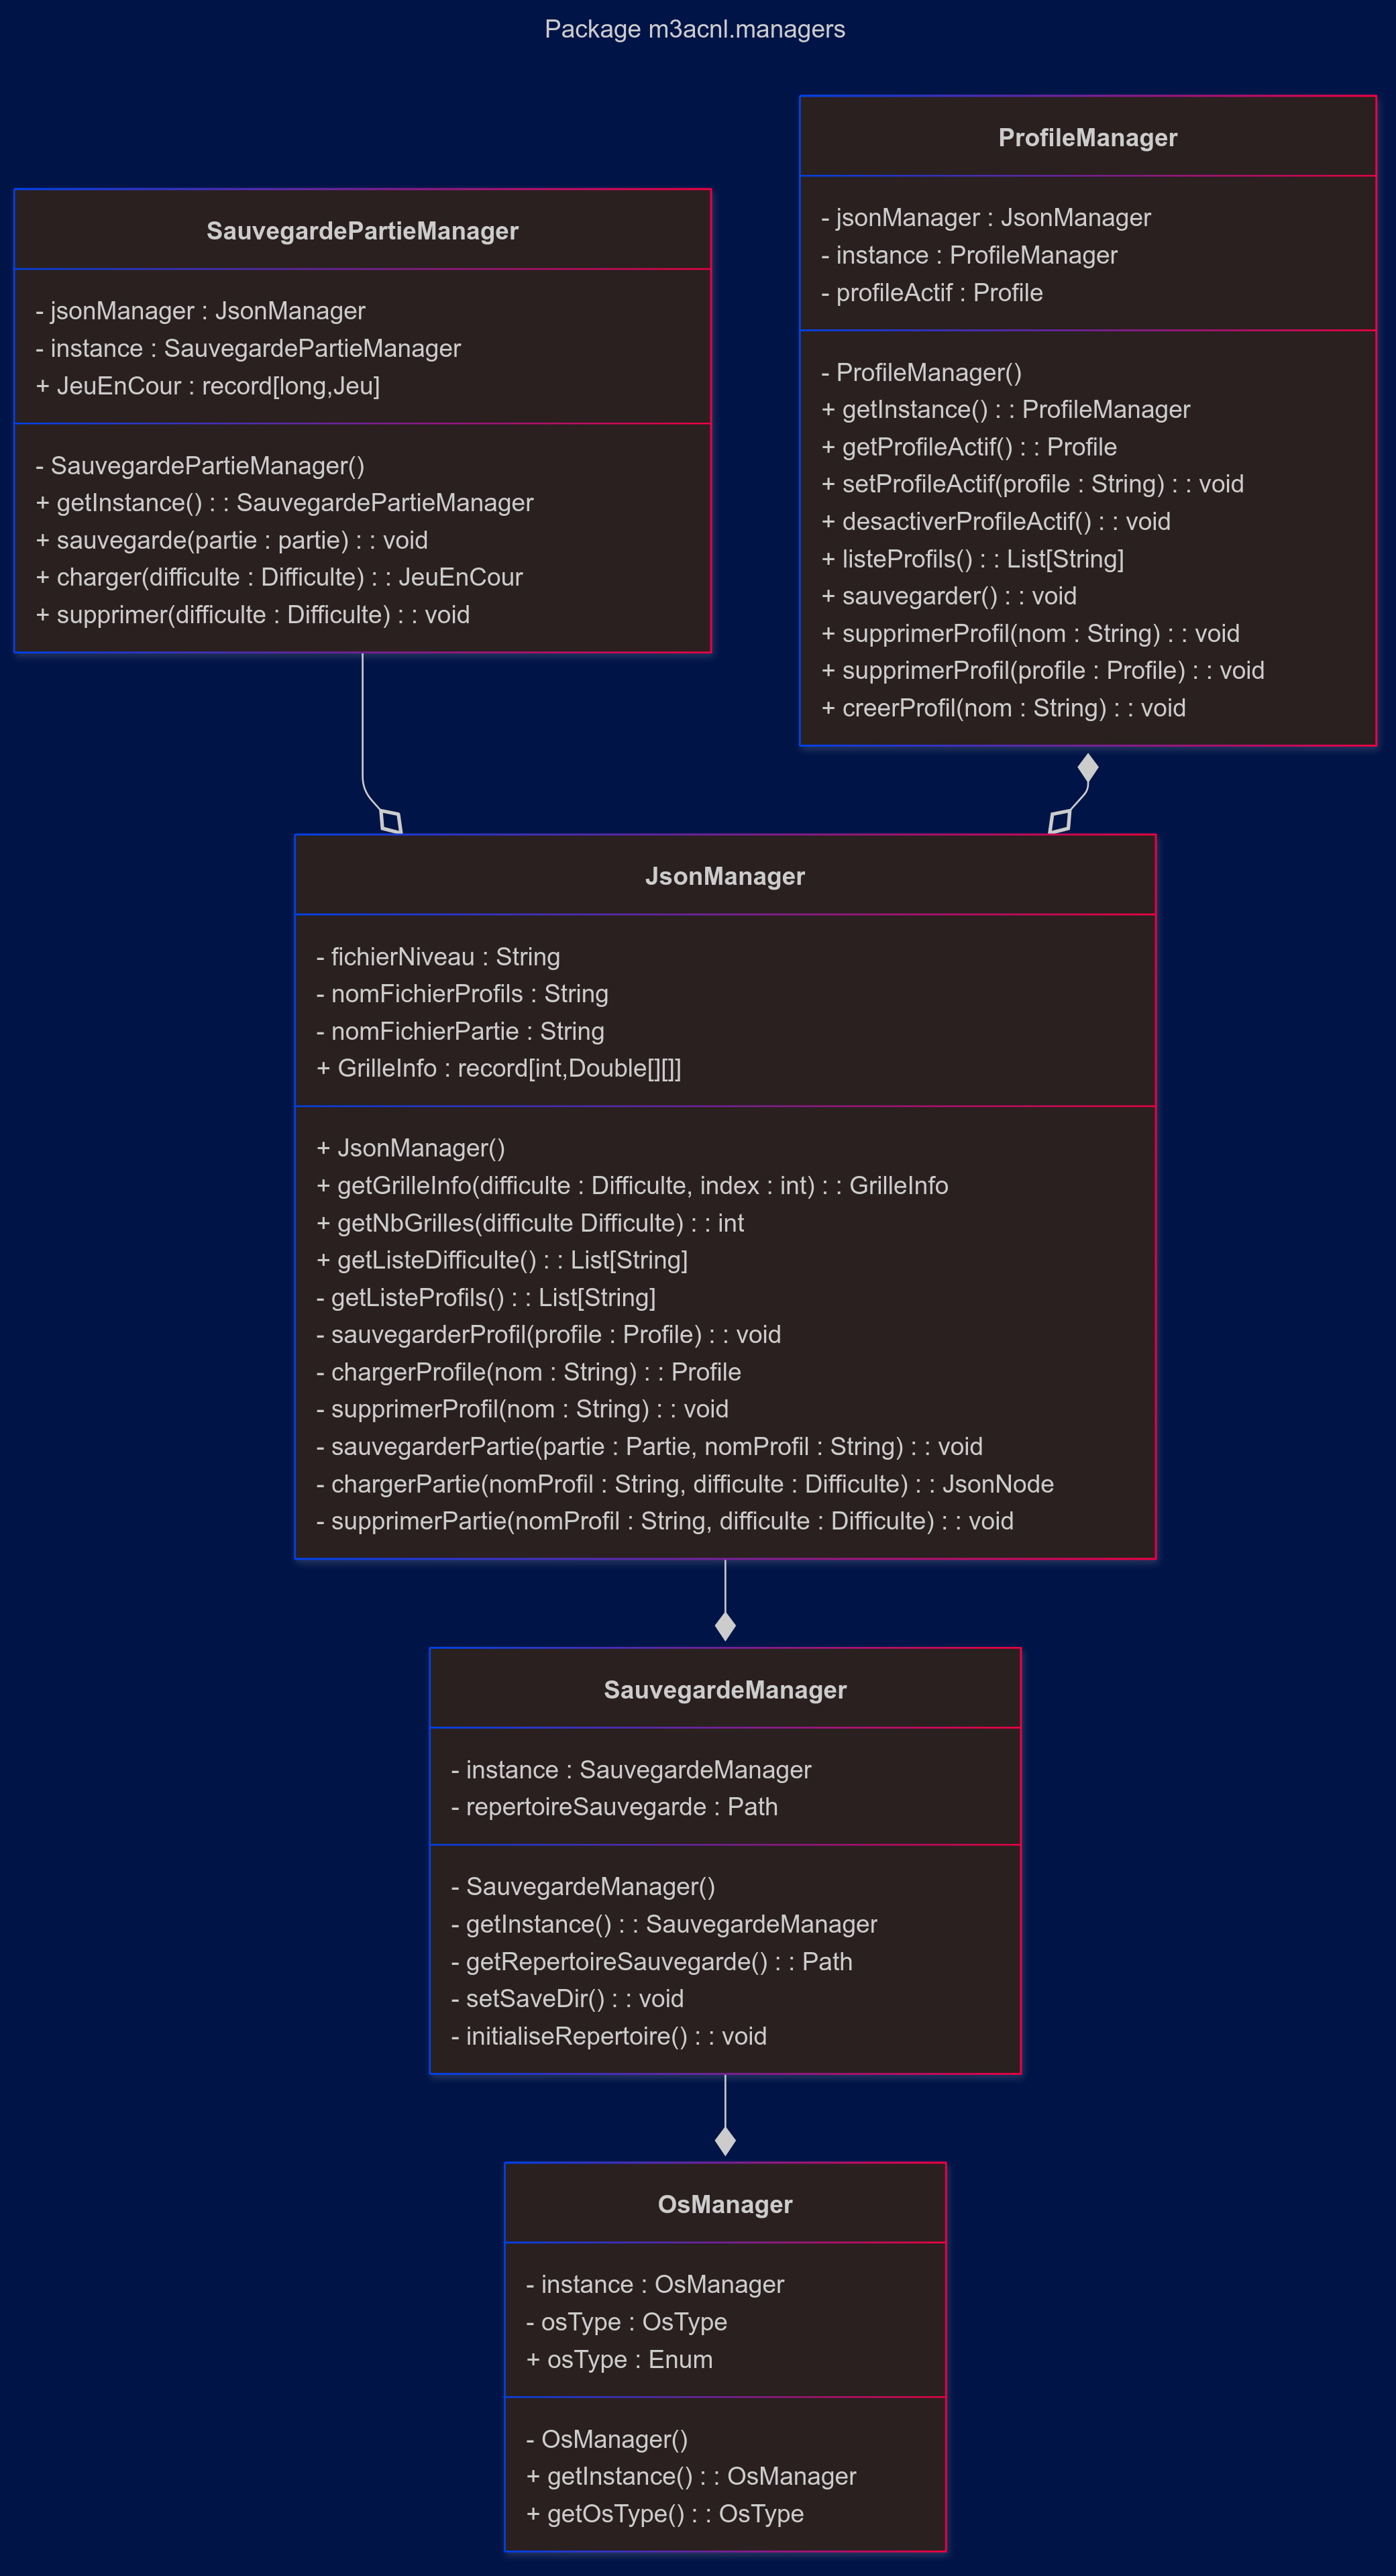
\includegraphics[width=\textwidth,height=\dimexpr\textheight-40pt\relax,keepaspectratio]{../Annexe/classes/managers.png}
\end{center}

\pagebreak

\textbf{Diagramme de classe des profils.}\\
\begin{center}
    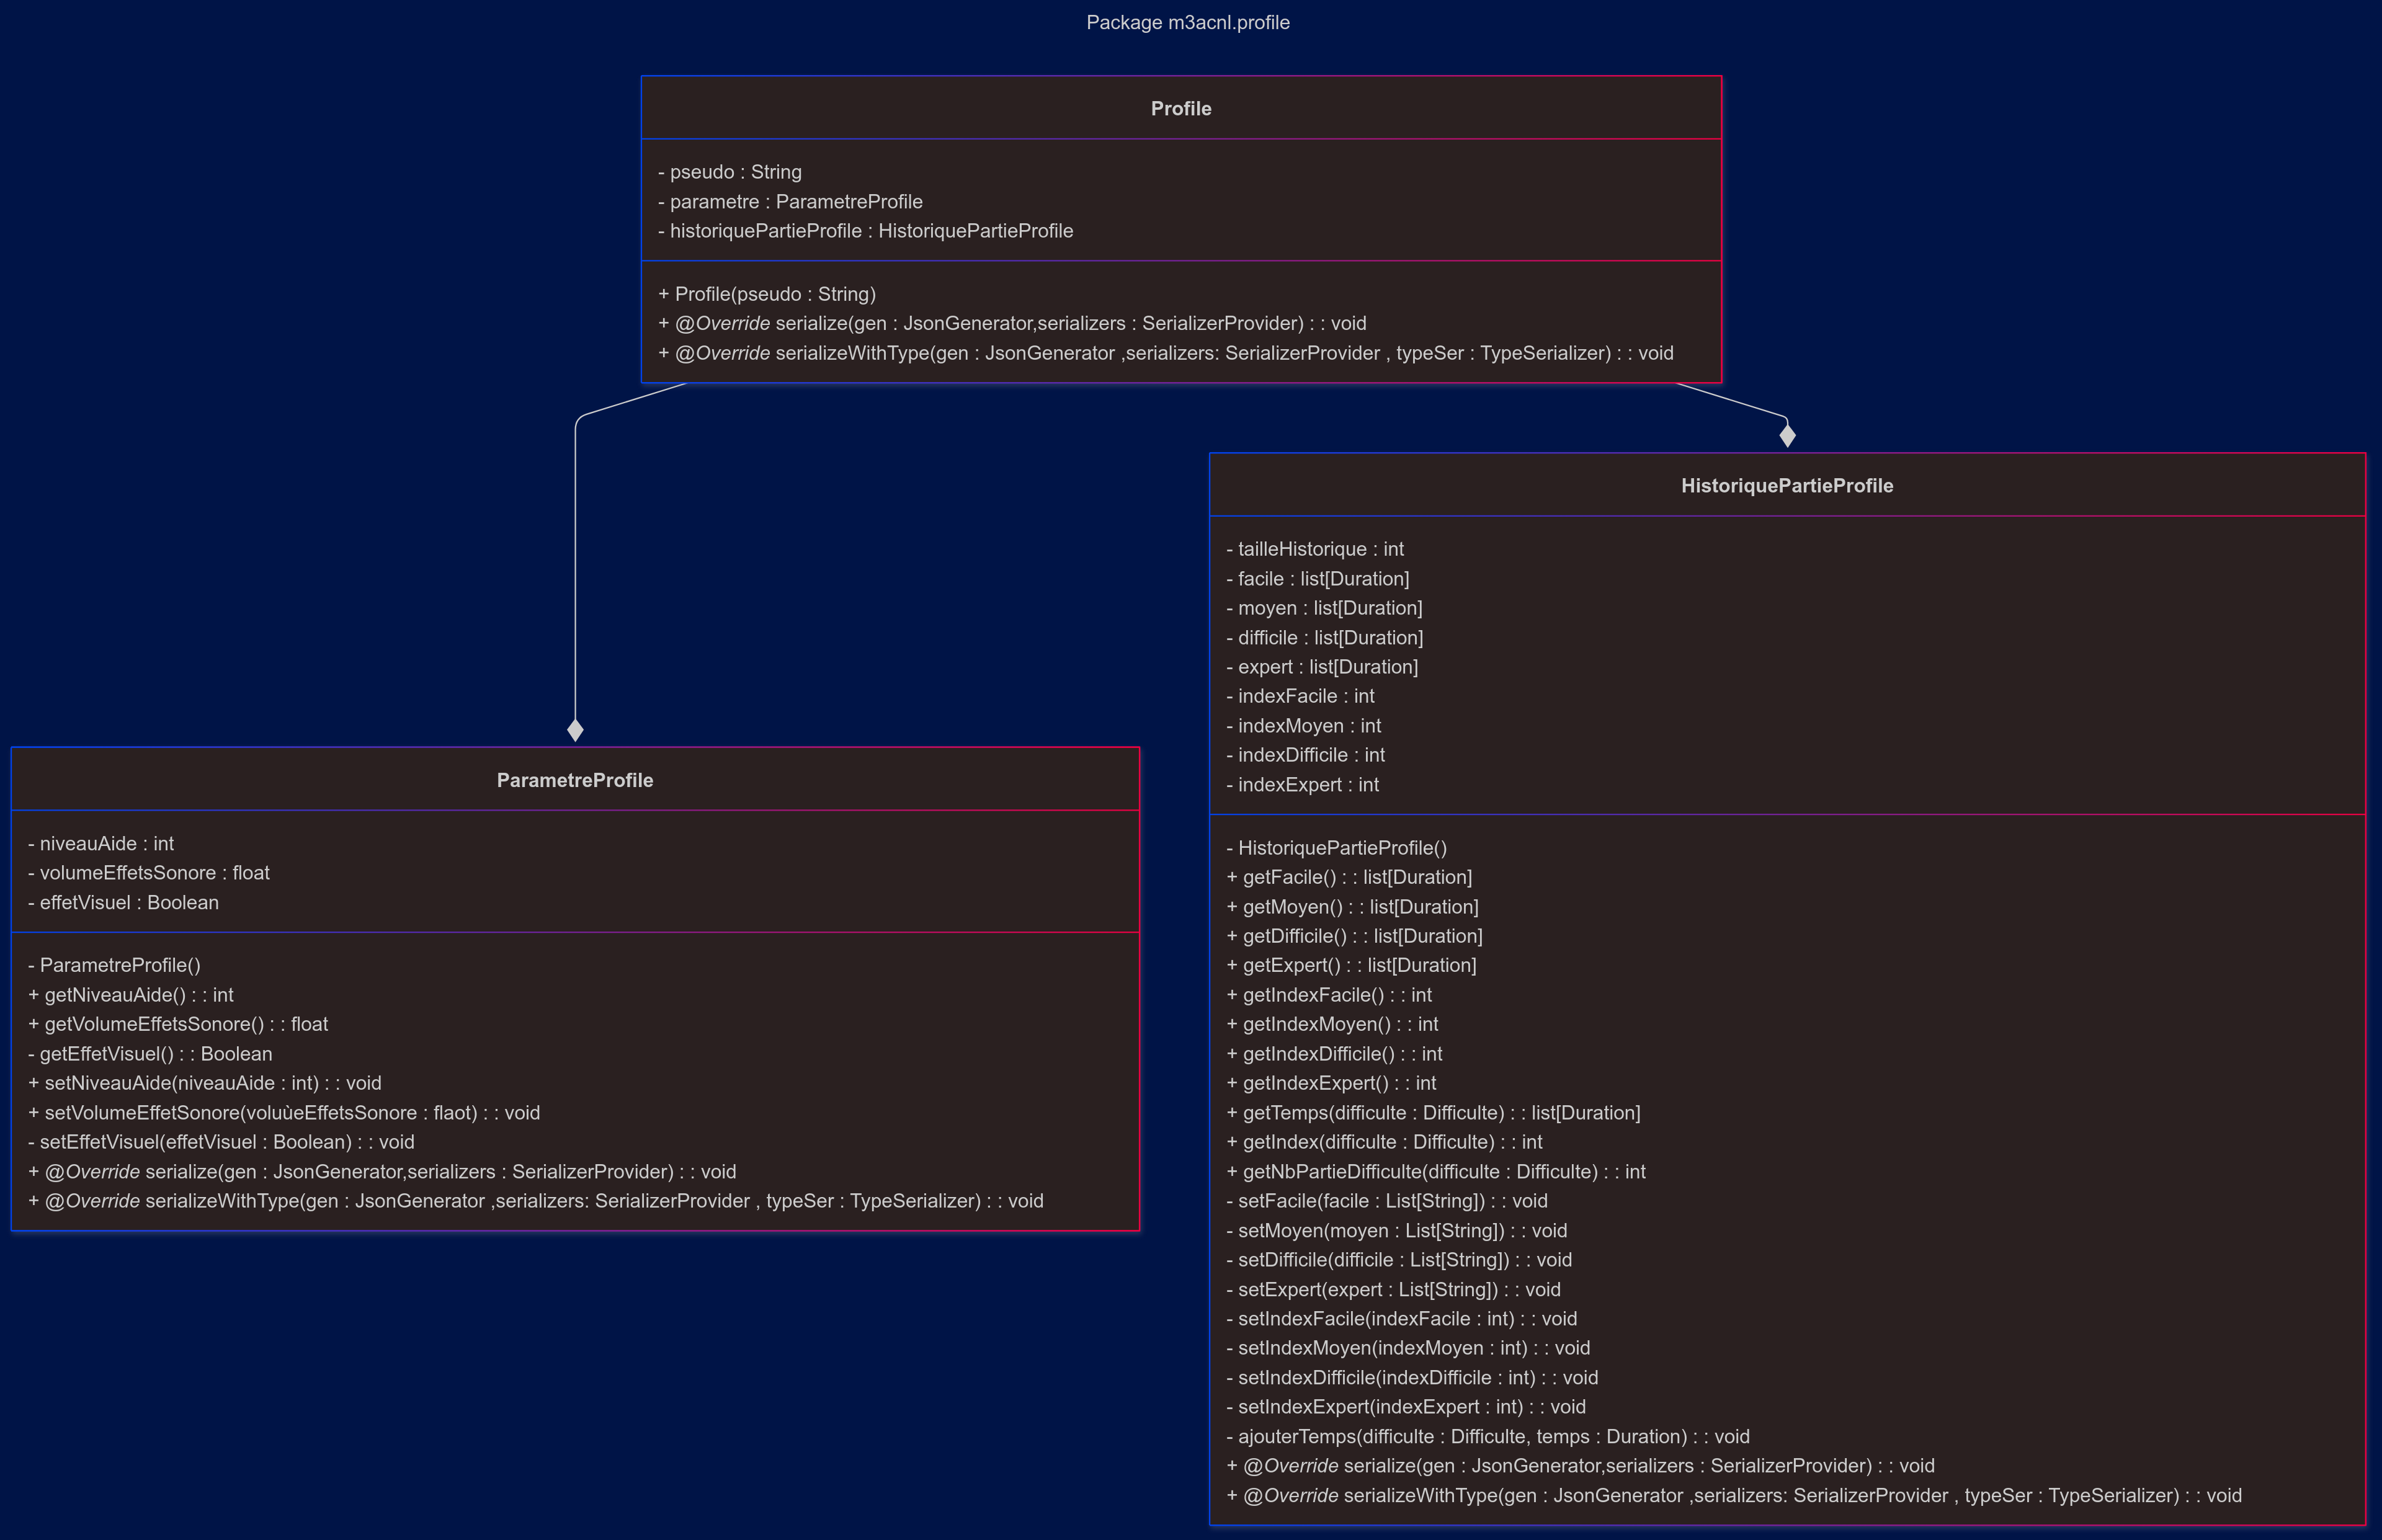
\includegraphics[width=\textwidth,height=\textheight,keepaspectratio]{../Annexe/classes/profile.png}
\end{center}

\pagebreak

\textbf{Diagramme de classe de la logique du jeu.}\\
\begin{center}
    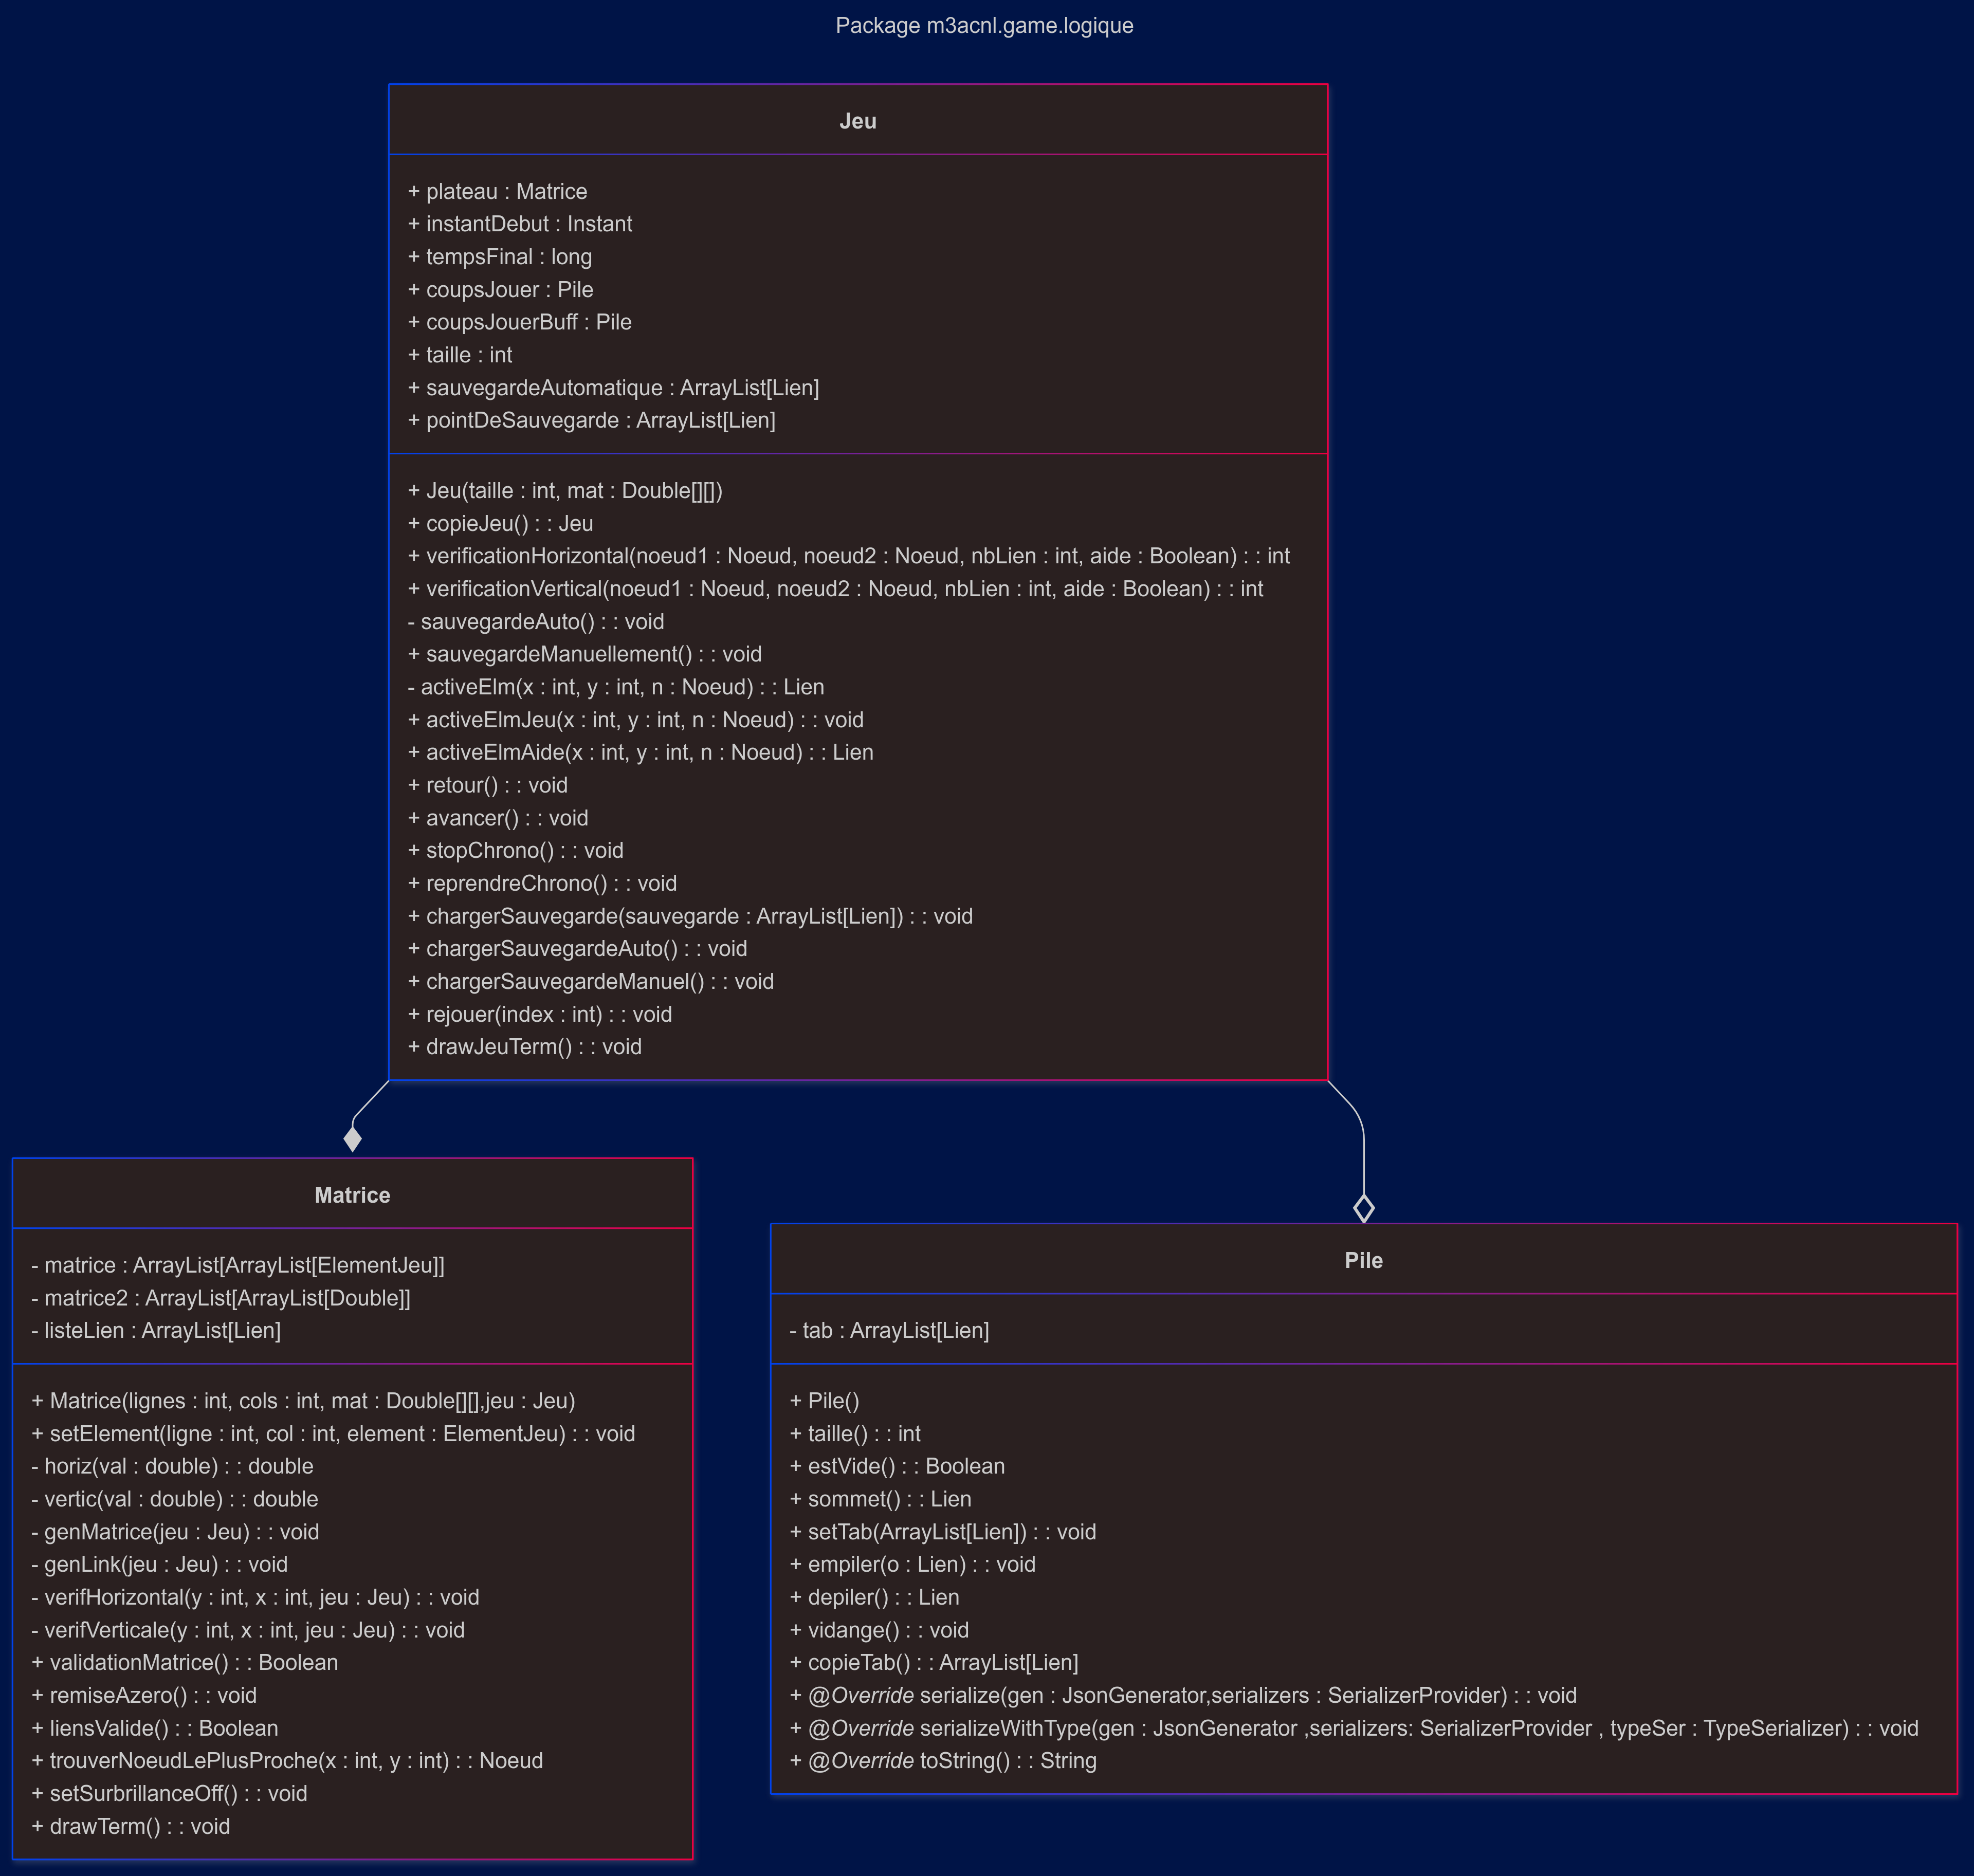
\includegraphics[width=\textwidth,height=\textheight,keepaspectratio]{../Annexe/classes/logique.png}
\end{center}

\pagebreak

\textbf{Diagramme de l'interface d'elementJeu.}\\
\begin{center}
    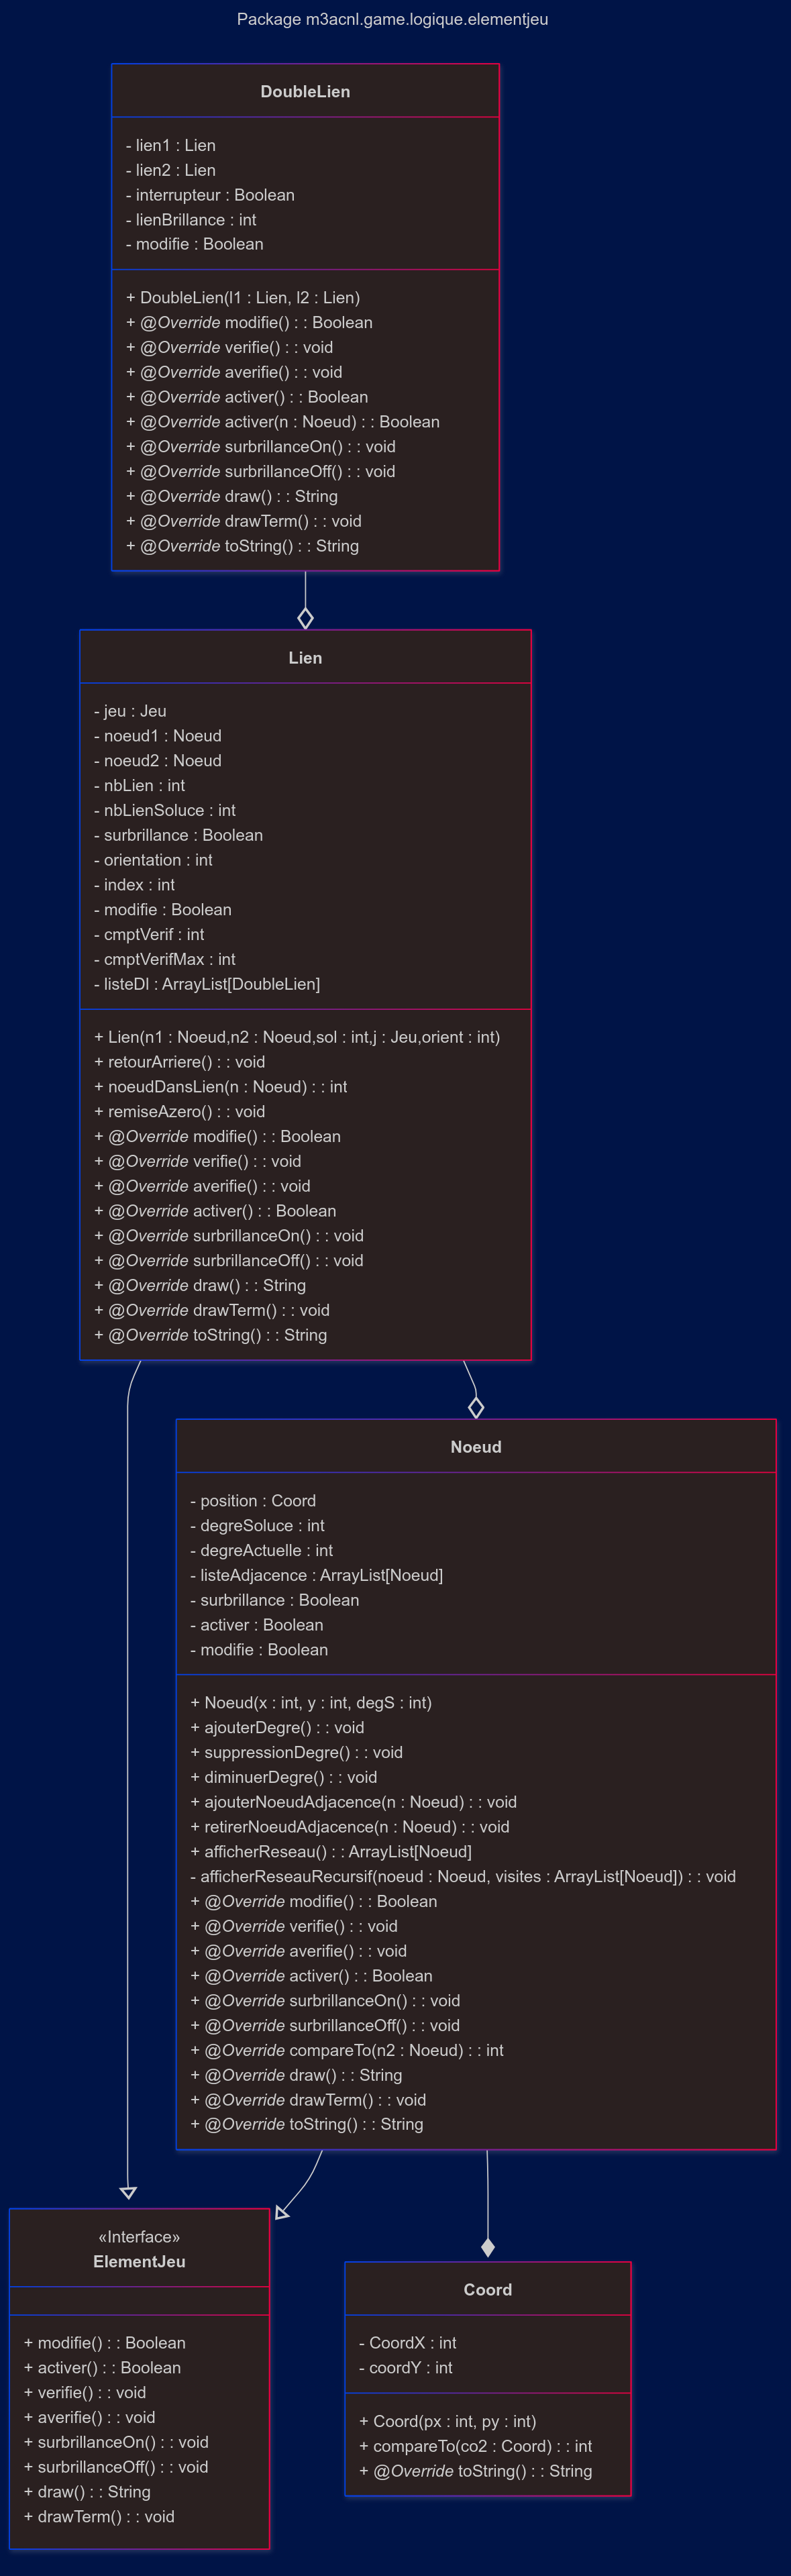
\includegraphics[width=\textwidth,height=\dimexpr\textheight-40pt\relax,keepaspectratio]{../Annexe/classes/elementJeu.png}
\end{center}

\pagebreak

\textbf{Diagramme de classe des aides.}\\
\begin{center}
    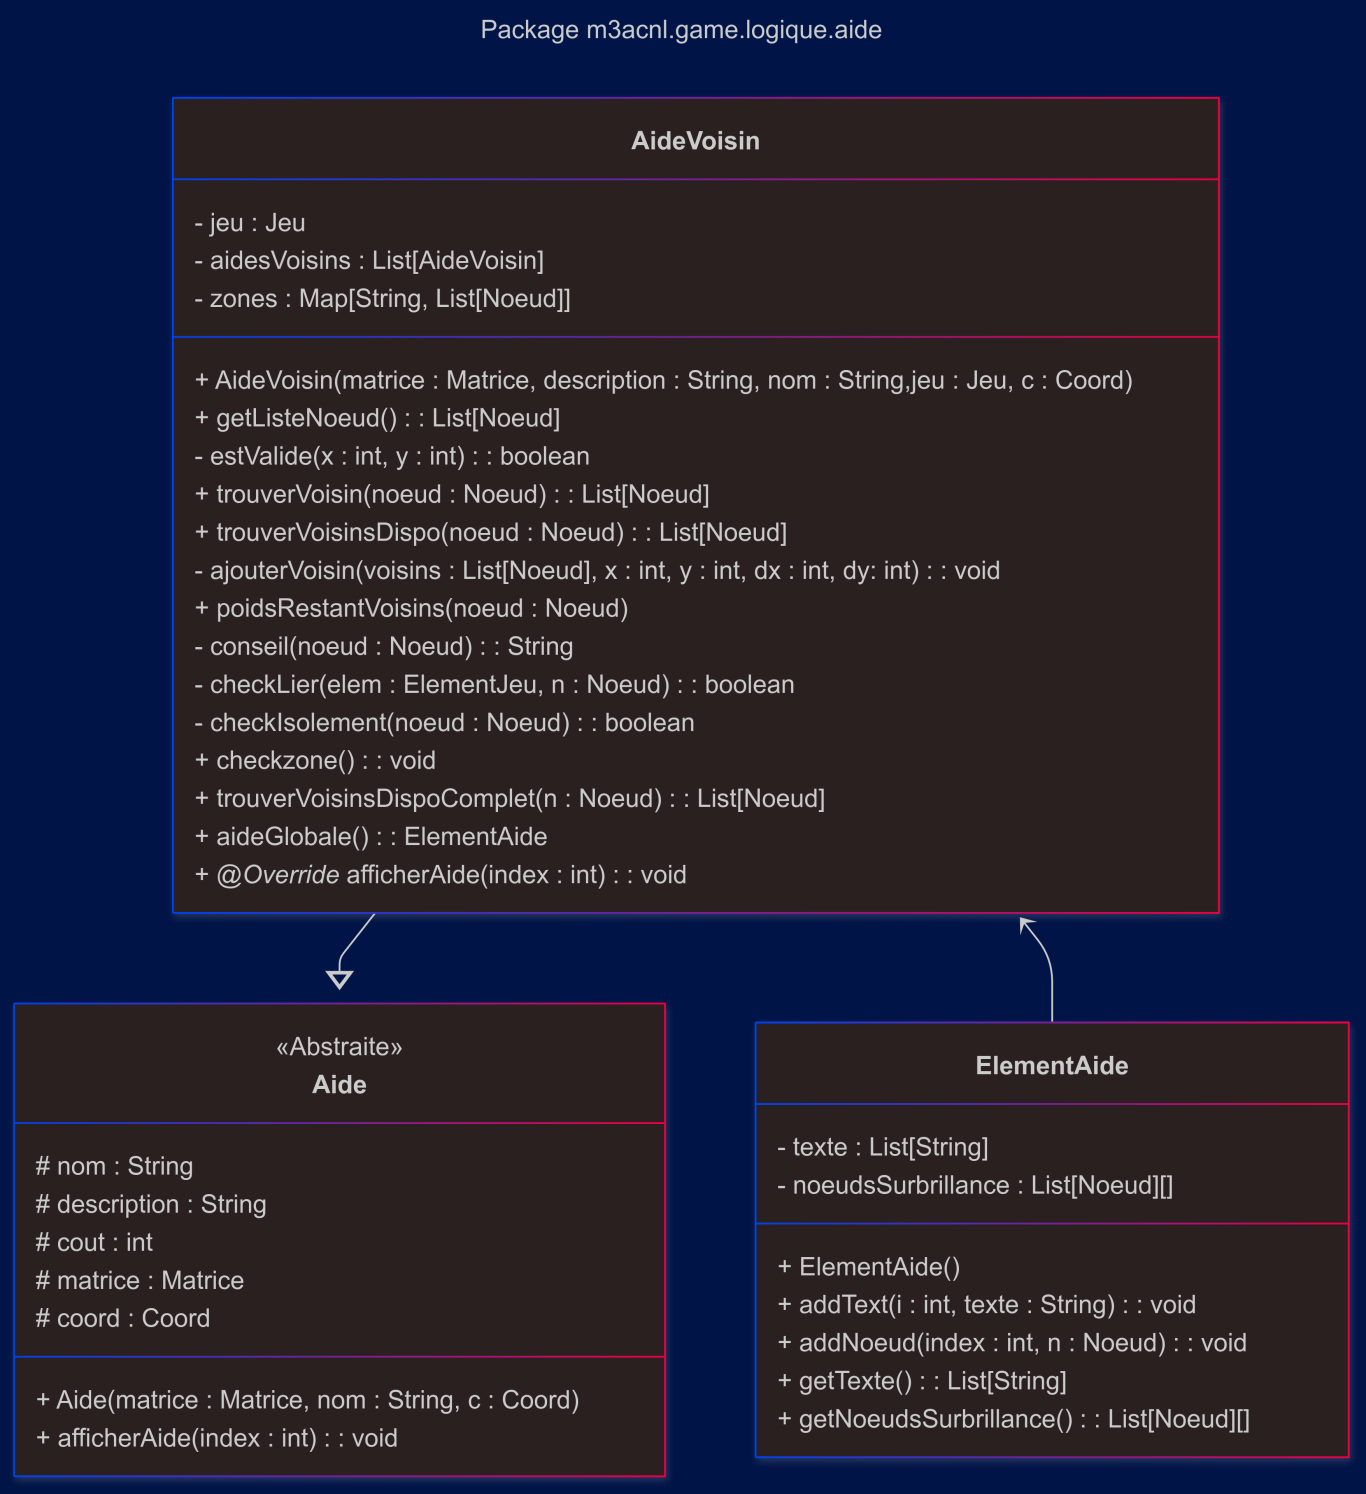
\includegraphics[width=\textwidth,height=\dimexpr\textheight-40pt\relax,keepaspectratio]{../Annexe/classes/aides.png}
\end{center}
